\documentclass[12pt]{article}

\usepackage{enumerate}
\usepackage{rotating}
\usepackage{multicol}
\usepackage{multirow}
\usepackage{graphicx}
\usepackage{fullpage}
\usepackage{subfigure}
\usepackage{setspace}
\usepackage{listings}
\usepackage{lastpage}

\graphicspath{{./images/}}

% for references
\usepackage[pagebackref=false,colorlinks,linkcolor=blue,citecolor=magenta]{hyperref}
\usepackage[nottoc]{tocbibind}
\usepackage{fancyhdr}
\setlength{\headsep}{25pt}

\pagestyle{fancy}
\fancyhf{}
\lhead{\lr{Digital Image Processing}}
\rhead{تمرین چهارم}
\cfoot{صفحه \thepage\ از \pageref{LastPage}}
\lfoot{نیمسال مهر 00-99}
\rfoot{حمیدرضا ابوئی مهریزی}


% xepersian
\usepackage[extrafootnotefeatures]{xepersian}
\settextfont[Scale=1.4]{B Nazanin}
\setlatintextfont{Times New Roman}

\renewcommand{\labelitemi}{$\bullet$}

\begin{document}
	\doublespacing
	\begin{titlepage}
		\paragraph*{}
		\centering
			
			
			{\small به نام او}\\
			\vspace{1cm}
			\includegraphics[width=0.12\paperwidth]{aut.png}
			\hspace{1cm}
			\includegraphics[width=0.15\paperwidth]{DIP}
			\hspace{1cm}
			\includegraphics[width=0.12\paperwidth]{bme}\\
			\vspace{2cm}
			{\Huge پردازش تصویر}\\
			\vspace{2cm}
			{\large استاد : دکتر حامد آذرنوش}\\
			\vspace{0.5cm}
			{\small  دانشجو :‌ حمیدرضا ابوئی}\\
			\vspace{0.5cm}
			{\small شماره دانشجویی : 9733002}\\
			\vspace{0.5cm}
			{\small تمرین چهارم}\\
			\vfill
			{\tiny نیمسال مهر 00-99}
	\end{titlepage}
	\thispagestyle{plain}
	\tableofcontents
	\newpage
	%\onehalfspacing
	\doublespacing
	\section{سوال اول}
		\subsection{توضیحات تکمیلی روند کد}
		برای یافتن مقدار مناسب برای ورودی 
		\lr{balance}
		راهی که در کد موجود است به این صورت است که تصویر اصلی بدون بلور را با تصویر بازسازی شده با مقادیر مختلف
		\lr{balance}
		 مقایسه می‌کنیم. و هر مقداری که بیشترین تشابه به آن را داشته باشد به عنوان مقدار بهینه انتخاب می‌کنیم. 
		 
		 بدین منظور برای محاسبه ی بهینه تر این کار در دو مرحله و در هر مرحله محاسبات دقیق تر شده است . ابتدا فاصله ی بین ۰ تا 5.0 به ۱۰ قسمت تقسیم شده و مقدار بهینه در می آید سپس حدود عدد به دست آمده را مجددا بررسی میکنیم تا عدد مناسب تر به دست بیاید . برای مقایسه نیز از یافتن کمترین میانگین مربع خطا استفاده شده است.
	
	در تصاویر خروجی بیشتر و کمتر از 
	\lr{balance}
	نمایش داده شده است .
	
	در مکان اگر مقدار 
	\lr{balance}
	بیشتر باشد 
	میزان رینگینگ آن قوی تر است و دقت آن کمتر است 
	در فرکانس نیز میزان فرکانسش کمتر است .
	اگر مقدار آن نیز کمتر باشد فرکانس بیشتری خواهد داشت ولی میزان 
	\lr{accuracy}
	آن بیشتر خواهد شد 
	
		\subsection{ورودی برنامه}
		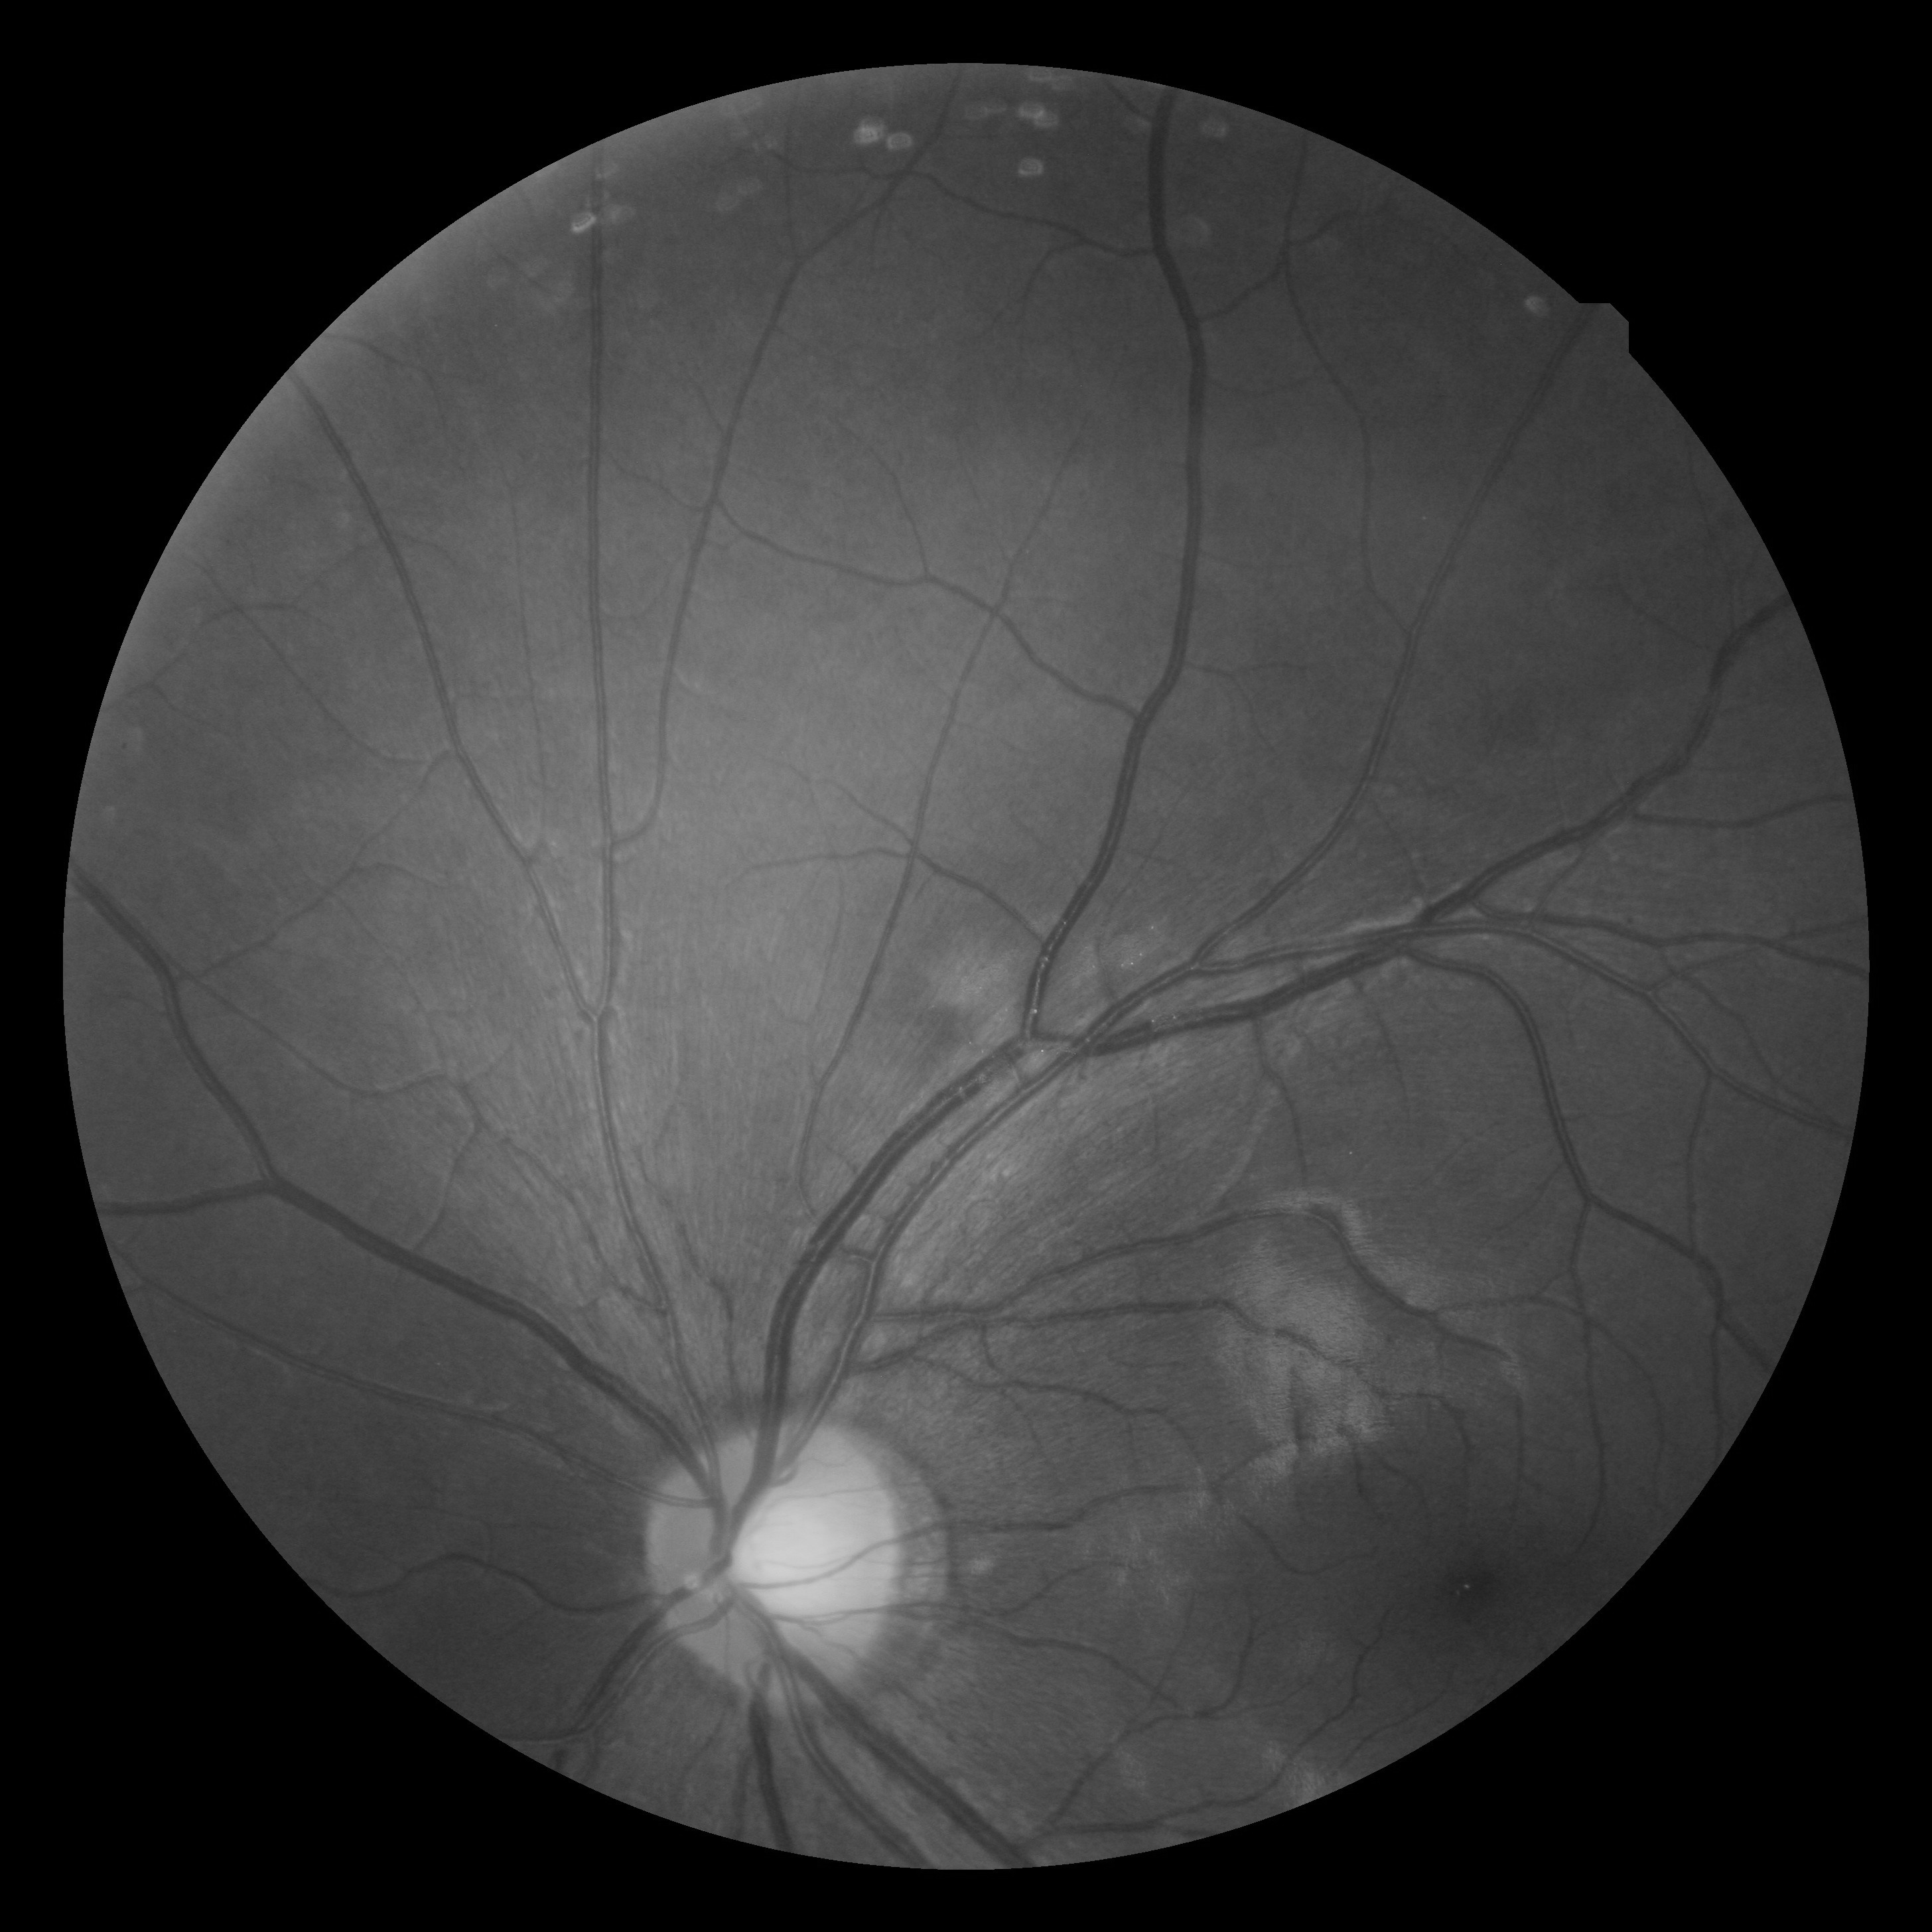
\includegraphics[width=5cm]{inputs/retina}
		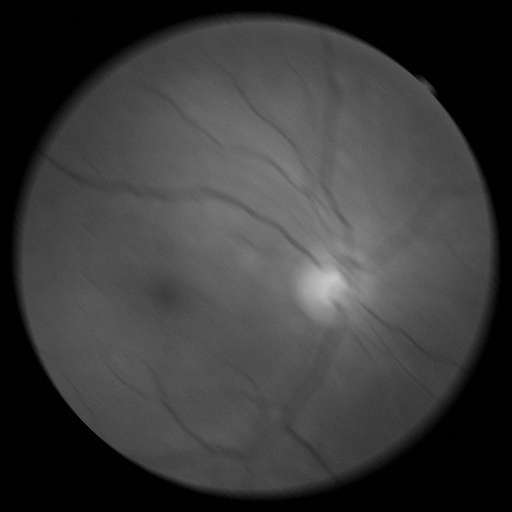
\includegraphics[width=5cm]{inputs/retina_motionblurred}
		\subsection{خروجی برنامه}
		
		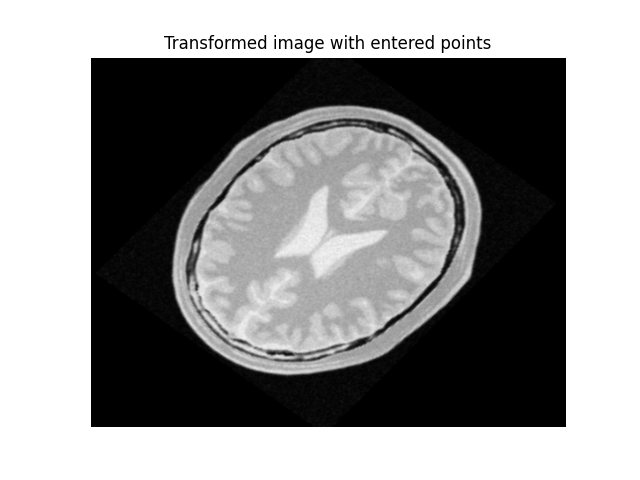
\includegraphics[width=17cm]{1}\\
		\includegraphics[width=17cm]{1-max}\\
		\includegraphics[width=17cm]{1-min}
		\newpage
		
			\doublespacing
		\section{سوال دوم}
		\subsection{توضیحات تکمیلی روند کد}
	عملیات 
	\lr{erosion }
	کرنل را داخل شکل میچرخاند و هر جا کاملا داخل قرار گرفت نقطه ی مرکز آن را جزو شکل در نظر میگیرد. بنابراین تصویر کوچک شده و نقاطی از نصویر که از ابعاد کرنل ما یعنی 15 کوچکتر باشد کاملا حذف میکند. 
	
	عملیات 
	\lr{dilation}
	روی تصویر اعمال میشود و هر جا که کرنل وارد به شکل شود آن را جزو شکل نهایی در نظر میگیرد یعنی تصویر بزرگ تر میشود و حفره هایی از تصویر را که کوچکتر از ابعاد کرنل باشد را حذف میکند .
	
	برای یافتن حداقل اندازه ی کرنل که تمام نویز های خارج از مستطیل را حذف کند با سعی و خطا به ابعاد 
	\lr{(29,52)\\(2,40)\\}
	میرسیم .
	
	البته این مستطیل ها باید به گونه ای انتخاب شوند که نویز های اطراف آن را به صورت کامل بگیرند.
		\subsection{ورودی برنامه}
		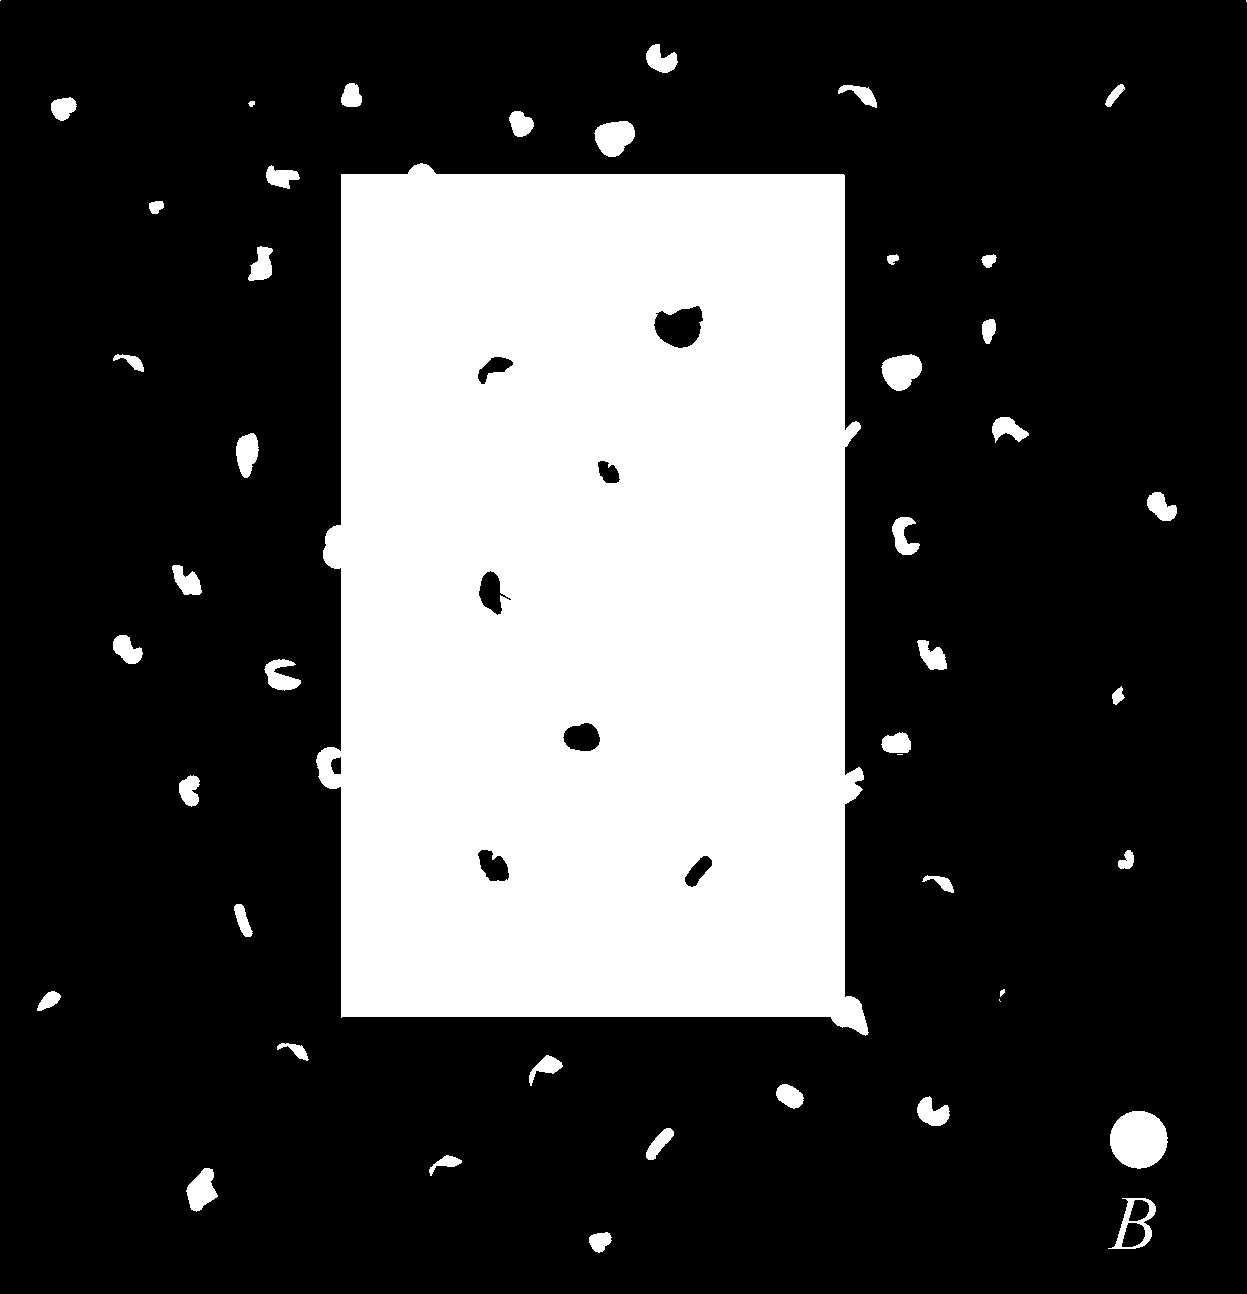
\includegraphics[width=5cm]{inputs/noisy_rectangle}
		\subsection{خروجی برنامه}
		
		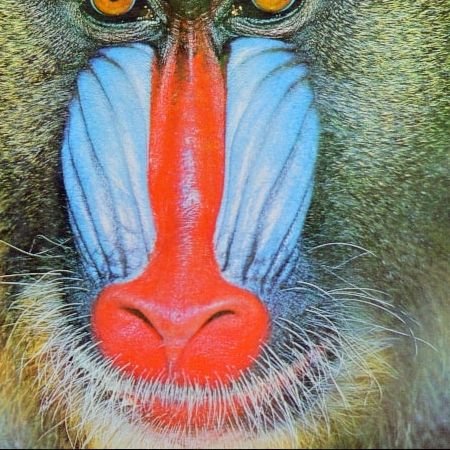
\includegraphics[width=10cm]{2}\\
		\includegraphics[width=10cm]{2-1}\\
		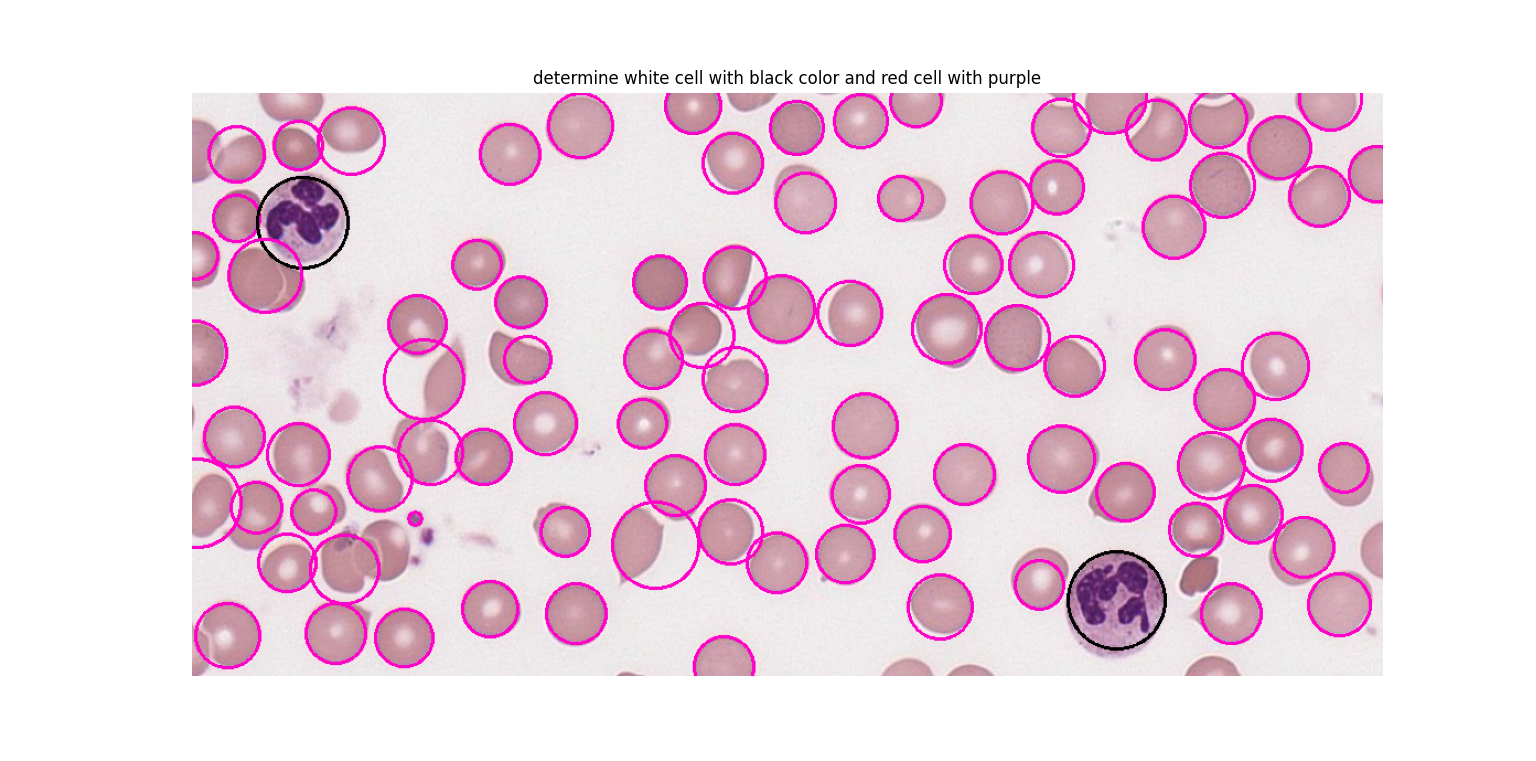
\includegraphics[width=10cm]{2-2}\\
		\includegraphics[width=10cm]{2-3}\\
		
		\newpage
		

\section{سوال سوم}
\subsection{توضیحات تکمیلی روند کد}
برای اثر انگشت ابتدا اوپنینک را اعمال میکنیم تا نویز های حذف شوند سپس از کلوزینگ استفاده میکنیم تا قطعاتی که از هم گسسته شدند به هم پیوندند و مسیر ها مشخص تر شوند

برای دومی هنگامی که کرنل کوچکتری را انتخاب میکنیم موقع گرادیان گرفتن یعنی هنگام ایروژن و دایلیشن تفاوتشان بیشتر میشود و بنابراین مرز آن کلفت تر می‌شود.

در برنج نیز ابتدا گرادیان بکگراند را با استفاده از حذف دانه ها با استفاده از ایرود کردن تصویر با کرنل بزرگ تر از اندازه ی دانه برنج می یابیم و آن را از تصویر خود کم می کنیم . حال با یک ترشهولد ساده میتوان دانه های برنج را کاملا مشخص کرد.


\subsection{ورودی برنامه}
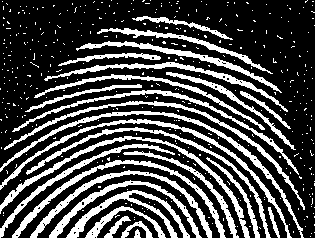
\includegraphics[width=5cm]{inputs/fingerprint}
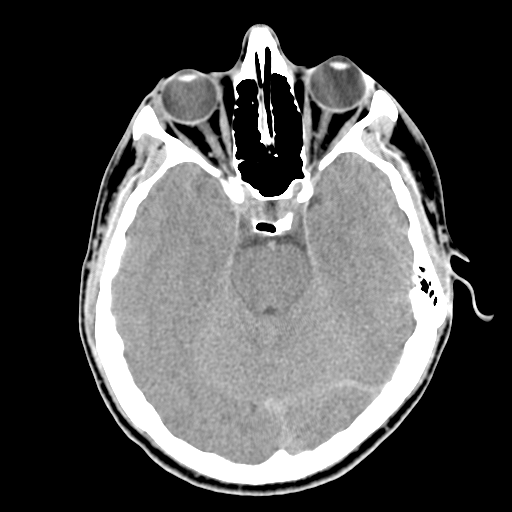
\includegraphics[width=5cm]{inputs/headCT}
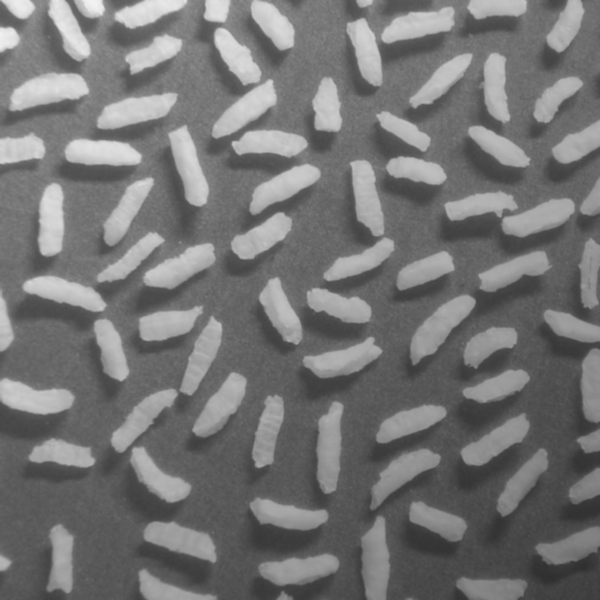
\includegraphics[width=5cm]{inputs/rice}
\subsection{خروجی برنامه}

\includegraphics[width=10cm]{3}\\
\includegraphics[width=10cm]{3-1}\\
\includegraphics[width=10cm]{3-2}\\
\includegraphics[width=10cm]{3-3}\\

\newpage

\end{document}
